\documentclass{article}
\usepackage{tbil-de}
%\usetikzlibrary{external}
%\tikzexternalize 
%\tikzsetexternalprefix{aux/}
\usepackage[top=1in,bottom=1in,right=1in,left=1in]{geometry}

\parindent=0pt
\parskip=1em

%Problem environment -- takes an argument which is the standard
\newenvironment{problem}[1]
%before
{
  \begin{flushleft}
  %{\bfseries \arabic{problem} .}
  %Problem numbering by standard
  \textbf{#1}.
  \ignorespaces
}
%after
{
  \end{flushleft}
}

\newenvironment{solution}
%before
{
  \ignorespaces
  \textbf{Solution:}
}
%after
{
  \ignorespacesafterend
  \begin{flushright}
  {\bfseries \qed}
  \end{flushright}
}



\begin{document}

\begin{center}
\Large \textbf{Sample Assessment Exercises}
\end{center}

This document contains one exercise and solution for each standard.
The goal is to give you an idea of what the exercises might look like,
and what the expectations for a complete solution are.



\begin{problem}{C1}
Find the general solution to \[y'+y=-t^2.\]
\end{problem}
\begin{solution}
First, we find a general solution to the homogeneous equation (removing all non-\(y\) terms) 
\[y_h'+y_h=0.\]
Since this is a first-order constant coefficient ODE, we know the answer is a modification of
\(ke^x\). We find that \(y_h=ke^{-x}\) is valid, since
\[y_h'+y_h=\frac{d}{dx}[ke^{-x}]+ke^{-x}=-ke^{-x}+ke^{x}=0.\]

The simplest particular solution for this homogeneous ODE is \(y_0=e^{-x}\),
so we use variation of parameters by assuming there is a non-homogeneous particular solution
\(y_p=vy_0=ve^{-x}\) for some function \(v\) (which we now need to find).

Using the product rule we find \(y_p' = v'e^{-t}-ve^{-t}\), so we may substitute into the original ODE to find
\[y_p ' + y_p = (v'e^{-t}-ve^{-t}) + ve^{-t} = v'e^{-t}=-t^2.\]

Thus \(v'=-t^2e^t\), so (after integrating by parts twice) we conclude \(v=\int -t^2 e^t\ dt  = -t^2 e^t +2te^t-2e^t\).  
Thus \(y_p = ve^{-t} = (-t^2+2t-2)e^te^{-t}=-t^2+2t-2\), so the general solution is 
\[y=y_h+y_p=ke^{-t}-t^2+2t-2.\]
\end{solution}

%% Original solution using undetermined coefficients
%We can find a particular solution \(y_p\) to the given equation by using undetermined coefficients; since \(-t^2\) is a polynomial, we let \(y_p = At^2+Bt+D\) and determine the coefficients \(A\), \(B\), and \(D\).  

%\begin{align*}

%y_p ^\prime +y_p= &= (2At+B)+(At^2+Bt+D) \\

%&= At^2+(2A+B)+(B+D)

%\end{align*}

%

%So if \(y_p\) is a solution, we must have \(y_p ^\prime+y_p = -t^2\), giving us the system of equations

%\begin{align*}

%A&=-1 \\ 2A+B &= 0 \\ B+D&=0

%\end{align*}

%Thus we easily deduce that \(A=-1\), \(B=2\), and \(D=-2\), giving \(y_p = -t^2+2t-2\).  Thus, the general solution is

%\[y = -t^2+2t-2+ce^{-t}.\]



\begin{problem}{C2}
Consider the following scenario: 
A water droplet with a radius of \(10\ {\rm \mu m}\) has a mass of about \(4 \times 10^{-15} {\rm kg}\) 
and a terminal velocity of \(3\ {\rm \frac{cm}{s}}\).  The droplet is dropped from rest;
assume that acceleration due to gravity is given by \(9.8{\rm\frac{m}{s^2}}\).
\begin{enumerate}[(a)]
\item Write down an IVP modelling the velocity.
\item What is its velocity after \(0.01\ {\rm s}\)?
\end{enumerate}
\end{problem}
\begin{solution}
\begin{enumerate}[(a)]
\item 
%Let \(v\) be the velocity of the droplet.
%The total force \(F_t\) acting on the water droplet is the sum of  gravity \(F_g\) and air resistance \(F_r\).
%\[F_t=F_g+F_r\]
%The total force is given by mass times the accleration \(v'\): \(F_t=mv'\).
%The force of gravity is given by mass times acceleration due to gravity, negative as it oriented downwards: \(F_g=-mg\).
%In a water droplet this size, air resistance is proportional to its velocity, \(F_r=-bv\) for a drag coefficient \(b>0\).
%
The ODE modeling the velocity of a tiny mass under gravity and air resistence
is \(mv'=-mg-bv\)
where \(m\) is the mass and \(g\) is the acceleration due to gravity, both given.
The coefficient of air resistence \(b\) is not given.
Since the object is dropped from rest, we know \(v=0\) when \(t=0\). So the initial value problem is given by
\[mv'=-mg-bv\hspace{3em}v(0)=0\]

To find \(b\), we note that the given terminal velocity 
\(v_t\) occurs when
there is no acceleration: \(v'=0\). So we may solve
\[0=-mg-bv_t\]
to get \(b=-\frac{mg}{v_t}\). Thus the simplified IVP is given by
\[v'-av=-g\hspace{3em}v(0)=0\]
where \(a=\frac{g}{v_t}\).

\item To solve for \(v\), we first solve the homogeneous system
\[v_h'-av_h=0\]
which has the general solution \(v_h=ke^{at}\), and a simple
particular solution \(v_0=e^{at}\). So we use varation of parameters to
assert that \(v_p=wv_0=we^{at}\) is a particular solution for the original equation.
If so, then \(v_p'=w'e^{at}+awe^{at}\) and thus
\[v_p'-av_p=w'e^{at}+awe^{at}-awe^{at}=w'e^{at}=-g\]
and therefore \(w'=-ge^{-at}\). By integration, \(w=\frac{g}{a}e^{-at}\)
and thus \(v_p=\frac{g}{a}\).

Therefore the general solution is given by \(v=v_h+v_p=ke^{at}+\frac{g}{a}\).
Using the initial condition \(v(0)=0\), we have \(0=ke^0+\frac{g}{a}\)
and thus \(k=-\frac{g}{a}\). So we have that \(v=-\frac{g}{a}e^{at}+\frac{g}{a}\)
or \(v=\frac{g}{a}(1-e^{at})\).
Thus our final answer is given by plugging in 
\[
g=9.8,\hspace{1em}
a=\frac{g}{v_t}=\frac{9.8}{-0.03}\approx-326.7,\hspace{1em}
t=0.01
\]
which yields the result \(v\approx -0.029\). So after 1/100 of a second,
the droplet is falling at a rate of about 29 millimeters per second.
\end{enumerate}
\end{solution}


\begin{problem}{C3}
Find the general solution to \[y''+6y'+13y=0.\]
\end{problem}
\begin{solution}
We begin by writing the auxilliary equation \(r^2+6r+13=0\) and finding the roots.  There are many ways to do this; here, we complete  the square:
\[0=r^2+6r+13=r^2+6r+9+4=(r+3)^2+4.\]
Thus, we can easily solve to obtain \(r=-3\pm2i\).  Thus the general solution is
\[ y= c_1 e^{-3t} \cos(2t) + c_2 e^{-3t} \sin(2t) .\]
\end{solution}

\begin{problem}{C4}
Find the solution to
\[
y'' + 10y' + 24y = 0
\]
when \(y(0)=-3\) and \(y'(0)=2\).
\end{problem}
\begin{solution}
The auxilliary equation is \(r^2+10r+24=0\), which has roots \(r=-6\) and \(r=-4\).  Thus, the general solution is of the form \(y=c_1e^{-4t}+c_2e^{-6t}\).  
\begin{align*}
-3 &= y(0) = c_1+c_2 \\
2 &= y'(0)  = -4c_1-6c_2 
\end{align*}
Solving this system yields \(c_1 =-8\) and \(c_2 = 5\), so the solution to the IVP is \[y=-8e^{-4t}+5e^{-6t}\]
\end{solution}



\begin{problem}{C5}
Find the general solution to \[y'' + 10y' + 24y = e^{-4t} 
\]
\end{problem}
\begin{solution}
First, we find a general solution to the homogenous equation \(y''+10y'+24y=0\).  We begin by writing the auxilliary equation \(r^2+10r+24=0\), which has roots \(r=-6\) and \(r=-4\).  Thus, the general solution is of the form \(y=c_1e^{-4t}+c_2e^{-6t}\). 

We use variation of parameters to find a particular solution, \(y_p=v_1e^{-4t}+v_2e^{-6t}\) for some functions \(v_1, v_2\).  We assume for convenience \(v_1'e^{-4t}+v_2'e^{-6t}=0\), so that \(y_p ' = -4v_1e^{-4t} - 6v_2 e^{-6t}\), and \(y_p '' = -4v_1' e^{-4t}+16v_1e^[-4t] -6v_2'e^{-6t}+36v_2e^{-6t}\).  Substituting into the original ODE and simplifying yields
\[e^{-4t}=y_p''+10y_p'+14y_p = -4v_1'e^{-4t}-6v_2'e^{-6t}.\]
Combining with our earlier assumption we have the system
\begin{align*}
v_1'e^{-4t}+v_2'e^{-6t}&=0 \\
-4v_1'e^{-4t}-6v_2'e^{-6t} &= e^{-4t}
\end{align*}
Multipy both equations by \(e^{4t}\) for convenience:
\begin{align*}
v_1'+v_2'e^{-2t}&=0 \\
-4v_1'-6v_2'e^{-2t} &= 1
\end{align*}
Then six times the first equation plus the second yields \(2v_1'=1\), so \(v_1=\int \frac{1}{2}\ dt = \frac{1}{2} t\).  Substituting back into the first yields \(v_2'=-\frac{1}{2}e^{2t}\), so \(v_2 = \int -\frac{1}{2}e^{2t}\ dt = -\frac{1}{4} e^{2t}\ dt\), and thus \[y_p = \frac{1}{2}t e^{-4t} -\frac{1}{4}e^{-4t},\]
and thus the general solution is 
\[ y = \frac{1}{2}te^{-4t} + c_1 e^{-4t} + c_2 e^{-6t}.\]

\end{solution}


\begin{problem}{C6}
Consider the following scenario:
A \(2 {\rm kg}\) mass is suspended by a spring (with spring constant \(8 {\rm kg /s^2}\)).  The mass is pulled down \(1 {\rm m}\) from its equillibrium position and released from rest.  
\begin{enumerate}[(a)]
\item Write down an IVP modelling the position of the mass.
\item How long does it take for the mass to return to its equillibrium point?
\end{enumerate}
\end{problem}
\begin{solution}
Let \(y\) denote the vertical distance from equillibrium; then the forces acting are gravity and the spring force, giving the ODE
\[my''=-ky.\]
Substituting in the values of the constants \(m=2\) and \(k=8\), we have
\[ 2y''+8y=0 .\]
Note that the initial conditions are \(y(0)=-1\) and \(y'(0)=0\), so an IVP model is 
\[ 2y''+8y=0 \hspace{5em} y(0)=1,\ y'(0)=0.\]
Simplifying, we have \(y''+4y=0\), so the general solution is \(y=c_1 \cos(2t)+c_2\sin(2t)\).  The initial conditions are \(y(0)=-1\) and \(y'(0)=0\), which imply \(c_1=-1\) and \(c_2=0\), so the system is modelled by \(y=-\cos(2t)\).  This is first zero when \(2t=\frac{\pi}{2}\), i.e. when \(t=\frac{\pi}{4}\).  Thus the mass takes \(\frac{\pi}{4}\) {\rm s} to return to its equillibrium point.
\end{solution}




\begin{problem}{F1}
Sketch a solution curve through each point marked in the slope field.

\begin{center}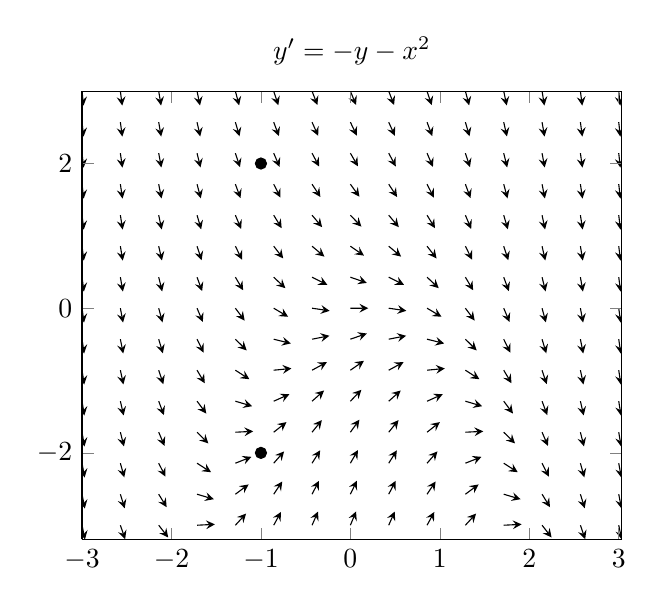
\begin{tikzpicture}
    \begin{axis}[
        title={\(y' = -y -x^2 \)},
        domain=-3:3,
        view={0}{90},
        axis background/.style={fill=white},
    ]
        \addplot3[black,
            quiver={
             u={1/(sqrt(1 + (-y -x*x)^2))},
             v={(-y - x*x)/(sqrt(1 + (-y - x*x)^2))},
             scale arrows=0.2,
            },
            -stealth,samples=15]
                {exp(-x) - 1/2*sin(x) - 1/2*cos(x)};
        %KAWWWWWWW
        % Here be some points added to the swoopy loop vector fieldamagigs
        \addplot[mark=*] coordinates {(-1,2)}; % Obvious ordered pair for lococation
        \addplot[mark=*] coordinates {(-1,-2)};
    \end{axis}
\end{tikzpicture}\end{center}
\end{problem}


\begin{solution}

\begin{center}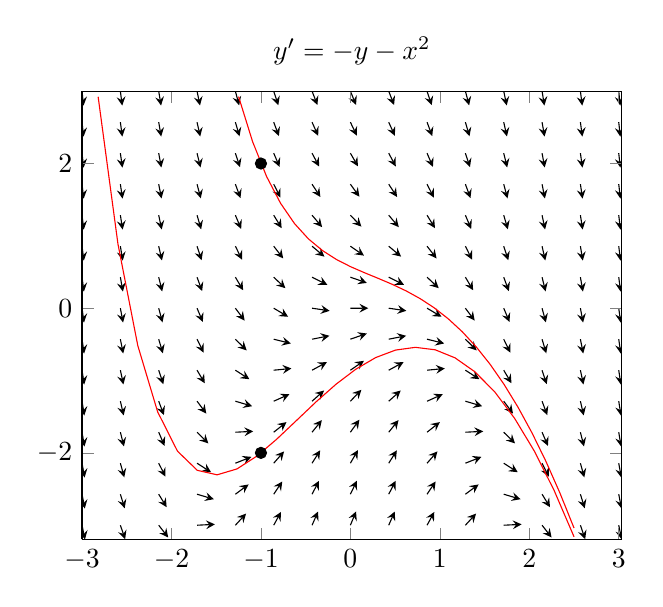
\begin{tikzpicture}
    \begin{axis}[
        title={\(y' = -y - x^2\)},
        domain=-3:3,
        view={0}{90},
        axis background/.style={fill=white},
    ]
        \addplot3[black,
            quiver={
             u={1/(sqrt(1 + (-y -x*x)^2))},
             v={(-y - x*x)/(sqrt(1 + (-y - x*x)^2))},
             scale arrows=0.2,
            },
            -stealth,samples=15]
                {exp(-x) - 1/2*sin(x) - 1/2*cos(x)};
        %KAWWWWWWW
        % Here be some points added to the swoopy loop vector fieldamagigs
        \addplot[mark=*] coordinates {(-1,2)}; % Obvious ordered pair for lococation
		\addplot[red,domain=-1.25:2.5] {-x^2+2*x-2+7/exp(1)*exp(-x)};
        \addplot[mark=*] coordinates {(-1,-2)};
		\addplot[red,domain=-2.82:2.5] {-x^2+2*x-2+3/exp(1)*exp(-x)};
    \end{axis}
\end{tikzpicture}\end{center}
\end{solution}


\begin{problem}{F2}
Solve \(y'+xy=x\).
\end{problem}
\begin{solution}
Rearranging, we have \(y'=x-xy=x(1-y)\), so we see the equation is separable, and write
\[ \frac{y'}{1-y} = x .\]

Thus we compute \(\int \frac{y'}{1-y}\ dx = \int \frac{1}{1-y}\ dy = -\ln|1-y|+c_1\), and \(\int x\ dx = \frac{1}{2}x^2+c_2\).  
Thus, we have (letting \(c_3=c_2-c_1\)) \[-\ln|1-y|=\frac{1}{2}x^2+c_3.\]
Then exponentiating, we have (letting \(c_4=\pm e^{-c_3}\) ) \(1-y=c_4e^{-\frac{1}{2}x^2}\), so (with \(c=-c_4\) ) the general solution is   \[y=1+c e^{-\frac{1}{2}x^2}.\]
\end{solution}

\begin{problem}{F3}
A ball has a mass of \(0.1 {\rm kg}\) and a drag coefficient of \(0.001 {\rm kg/m}\).  It is thrown with a velocity of \(20 {\rm m/s}\). 
\begin{enumerate}[(a)]
\item Write down an IVP modelling the horizontal velocity of the ball (ignore any vertical movement in the ball).
\item How long does it take the ball to travel \(20 {\rm m}\)?
\end{enumerate}
\end{problem}
\begin{solution}
The only force acting on the ball is air resistance (drag), so we have
\[mv'=-bv^2.\]
Substituting in our constants (and dividing through by \(m\)), we have
\[v'=- 0.1v^2 .\]
The initial condition is that it is travelling \(20 {\rm m/s}\), i.e. \(v(0)=20\), giving the IVP 
\[v'=- 0.1v^2 \vspace{5em} v(0)=20.\]
Solving this separable ODE, we obtain \(v=\frac{20}{1+2t}\).  To model the position of the ball, we integrate again, obtaining \(x=\int \frac{20}{1+2t}\ dt = 10 \ln |1+2t| +C\); using \(x(0)=0\), we see \(C=0\).  Then we simply need to solve \(x(t)=20\), i.e. \(20=10\ln|1+2t|\), so \(t=\frac{1}{2}(e^2-1) \approx 3.19 {\rm s}\).
\end{solution}



\begin{problem}{F4}
Consider the autonomous equation 
\[\frac{dx}{dt} = x^2-1.\]  
\begin{enumerate}[(a)]
\item Find and classify the critical points.
\item Describe the long term behavior of the solution passing through the point \( x(4)=0 \).
\end{enumerate}
\end{problem}
\begin{solution}

Note that \(x^2-1=(x-1)(x+1)\), so there are equillibria solutions at \(x=1\) and \(x=-1\).  We can thus compute a number line for \(x'\):

\begin{center}
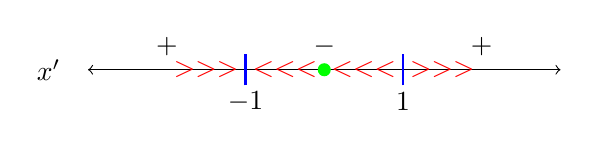
\begin{tikzpicture}
\node at (-3.5,0) {\(x'\)};
\draw[<->] (-3,0) -- (3,0);
\node at (-2,0.3) {\(+\)};
\node at (0,0.3) {\(-\)};
\node at (2,0.3) {\(+\)};
\draw[thick,blue] (-1,-0.2) -- (-1,0.2);
\node at (-1,-0.4) {\(-1\)};
\draw[thick,blue] (1,-0.2) -- (1,0.2);
\node at (1,-0.4) {\(1\)};
\node[red] at (-1.5,0) {\(>>>\)};
\node[red] at (-0.5,0) {\(<<<\)};
\node[red] at (0.5,0) {\(<<<\)};
\node[red] at (1.5,0) {\(>>>\)};
\node[fill,circle,green,scale=0.5] at (0,0) {};
\end{tikzpicture}
\end{center}

We see that \(-1\) is a sink (stable), while \(1\) is a source (unstable).  A trajectory passing through \(x(4)=0\) will approach \(x=-1\) in the limit.
\end{solution}

\begin{problem}{F5}
Solve \(y'+xy=x^3\).
\end{problem}
\begin{solution}
First, we solve the homogeneous equation \(y'+xy=0\), which is separable: \(\frac{y'}{y}=-x\), so \(\ln|y|=-\frac{1}{2}x^2+c\), or \(y=c_1e^{-\frac{1}{2}x^2}\). We then use variation of parameters to find a particular solution, writing \(y_p = v e^{-\frac{1}{2}x^2}\); substituting in and simplifying yields
\[x^3 = y_p ' +xy_p = v'e^{-\frac{1}{2}x^2} -vxe^{-\frac{1}{2}x^2} + xve^{-\frac{1}{2}x^2} = v'e^{-\frac{1}{2}x^2}.\]
Thus, \(v'=x^3 e^{\frac{1}{2}x^2} \).  This can be integrated by parts to obtain \(v=x^2e^{\frac{1}{2}x^2}-2e^{\frac{1}{2}x^2}\), so \(y_p = v e^{-\frac{1}{2}x^2} = x^2-2\).  Thus the general solution is
\[y=c_1e^{-\frac{1}{2}x^2} + x^2 - 2 .\]
\end{solution}

\begin{problem}{F6}
One of the two ODEs below is exact.  Identify which one, and solve it.
\begin{align*}
 (x + 3y)y'+y &=3x \\ %Exact
 (x + 3y)y'-y &=-3x  
\end{align*}
\end{problem}
\begin{solution}
Rewrite the first equation as \(y'=\frac{3x-y}{x+3y}\); if there is a function with \(\nabla F = \langle -(3x-y), x+3y\rangle\), then \[\frac{d}{dt}F(x,y)=\frac{\partial F}{\partial x} \frac{\partial x}{\partial t} + \frac{\partial F}{\partial y} \frac{\partial y}{\partial t} = -(3x-y)(x+3y)+(x+3y)(3x-y)=0,\] so \(F(x,y)=c\) is a solution of the autonomous system.

Note that  \(\langle -(3x-y), x+3y\rangle\) is conservative, as \(\frac{\partial}{\partial x}(x+3y)=1=\frac{\partial}{\partial y}(-3x+y)\); so a potential function \(F\) is found by integrating: \(F = \int x+3y\ dy = xy+\frac{3}{2}y^2+f(x) \), and differentiating with respect to \(x\), we have \(-3x+y=y+f'(x)\), so \(f'(x)=-3x\), in which case \(f(x)=\int -3x\ dx = \frac{-3}{2}x^2\), so a potential function is \(F(x,y)=xy+\frac{3}{2}y^2-\frac{3}{2}x^2\).  So the general solution to the ODE is
\[ xy+\frac{3}{2}y^2-\frac{3}{2}x^2 = c.\]
\end{solution}

\begin{problem}{S1}

\end{problem}
\begin{solution}

\end{solution}

\begin{problem}{S2}
Consider the following scenario:
Two competing fish species (red fish and blue fish) live in a lake.  In the absence of one species, the lake will support \(30,000\) of the other fish (as the species competes among itself for resources).  It is calculated that the competition coefficients are \(\alpha _{1,2}=\alpha _{2,1} = 0.5\).
\begin{enumerate}[(a)]
\item Write down a system of ODEs modelling the interaction of the two species.
\item If the lake is stocked with \(12,000\) blue fish and \(40,000\) red fish, what will happen to the populations in the long run?
\end{enumerate}
\end{problem}
\begin{solution}

\begin{align*}
x' &= \frac{r_1}{30000}x\left(30000-x-0.5y\right) \\
y' &= \frac{r_2}{30000}y\left(30000-y-0.5x\right) 
\end{align*}

Then the nontrivial isoclines are \(x+0.5y=30000\) and \(0.5x+y=30000\) which intersect at the (equillibrium) point \(20000,20000\).  Plotting the isoclines (TODO) shows that this a stable equillibrium (sink), so regardless of the intial populations, they will approach \(20,000\) of each species in the long run.

\end{solution}

\begin{problem}{S3}

\end{problem}
\begin{solution}

\end{solution}


\begin{problem}{N1}

\end{problem}
\begin{solution}

\end{solution}

\begin{problem}{N2}

\end{problem}
\begin{solution}

\end{solution}

\begin{problem}{N3}

\end{problem}
\begin{solution}

\end{solution}

\begin{problem}{N4}

\end{problem}
\begin{solution}

\end{solution}

\begin{problem}{N5}

\end{problem}
\begin{solution}

\end{solution}


\begin{problem}{D1}

\end{problem}
\begin{solution}

\end{solution}

\begin{problem}{D2}

\end{problem}
\begin{solution}

\end{solution}

\begin{problem}{D3}

\end{problem}
\begin{solution}

\end{solution}

\begin{problem}{D4}

\end{problem}
\begin{solution}

\end{solution}



\end{document}
